Um ein Bild von der allgemeinen Übereinstimmung der simulierten Daten mit den tatsächlich beobachteten Daten zu erhalten wird in diesem Kapitel das Jahresmittel der simulierten und beobachteten Daten verglichen. Dadurch erhält man einen Überblick über die geographische Übereinstimmung der Regenzonen und Trockengebiete im abgebildeten Bereich.
\begin{figure}[h]
	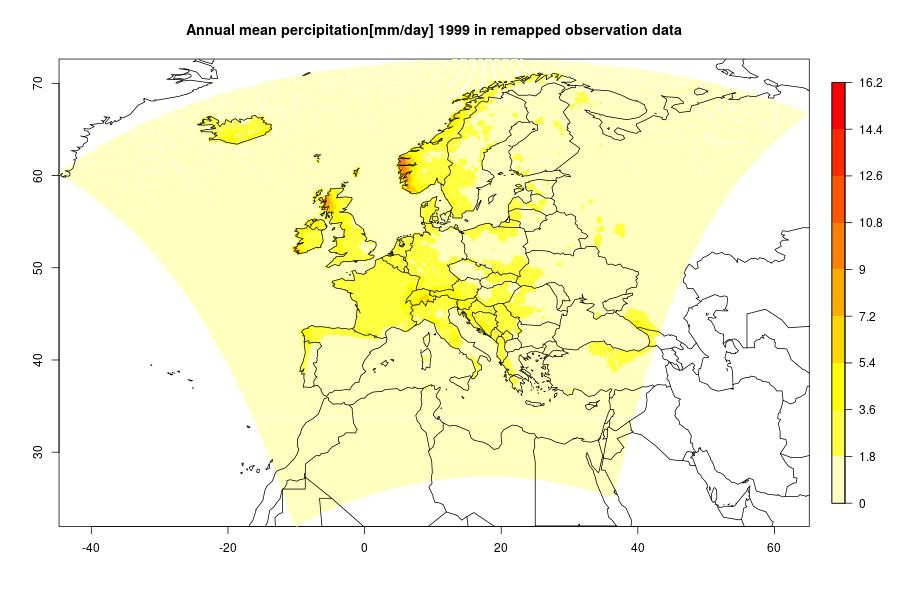
\includegraphics[width=15cm]{mean/mprs1999obs_remapped.jpg}
	\caption{Jährliches Mittel über den Niederschlag im Jahr 1999 der tatsächlich Beobachteten Daten}
	\label{fig:mobs99}
\end{figure}
\\
Zu Abb. \ref{fig:mobs99}: Man erkennt gut die starken Regenfälle an der Westküste Norwegens und Englands (bis zu 12.6 mm). Der Niederschlag an Irlands Westküste und im Alpenbereich fielen 1999 im Mittel schwach aus (bis zu 7.2mm). Über Deutschland, Frankreich und weiten Teilen Europas fielen im Schnitt 3.6-5.4 mm Regen am Tag.\\
\begin{figure}[h]
	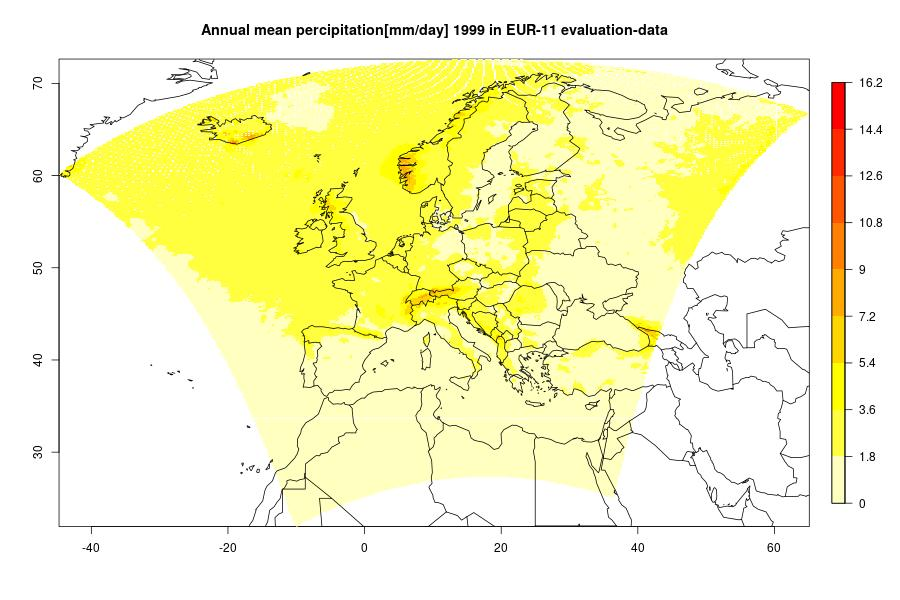
\includegraphics[width=15cm]{mean/msim1999eval.jpg}
	\caption{Jährliches Mittel über den Niederschlag im Jahr 1999 im evalualtion Datensatz von EUR-11}
	\label{fig:meval99}
\end{figure}
 \\
Zu Abb. \ref{fig:meval99}: Man sieht generell gute Übereinstimmungen an der Küste Norwegens und Englands, der Regen in Island und einigen Teilen des Alpenraumes fielen im Modell zu stark aus. Auch in Georgien am Kaukasus liefert das Modell einen zu starken Regen. Da das Klimamodell CCLM4-8-17 eine Parametrisierung der Konvektion vornimmt, ist die geringe Übereinstimmung in gebirgigen Gebieten nicht überraschend. Der Unterschied zur folgenden Abbildung \ref{fig:mhist99} ist lediglich die Quelle der Daten für das downscalen: hier wurde das CCLM mit Re-Analysedaten betrieben, im folgenden mit dem GCM MPI-ESM-LR.\\

\begin{figure}[h]
	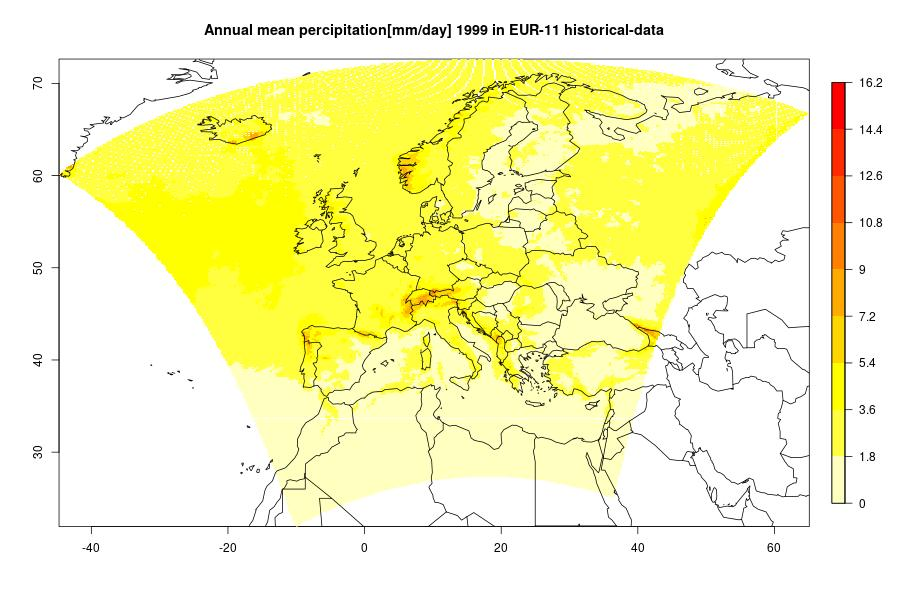
\includegraphics[width=15cm]{mean/msim1999hist.jpg}
	\caption{Jährliches Mittel über den Niederschlag im Jahr 1999 im historical Datensatz von EUR-11}
	\label{fig:mhist99}
\end{figure}
Zu Abb. \ref{fig:mhist99}: Der Regen an der norwegischen Westküste fällt bei dieser Modellaufnahme um einiges schwächer aus als in der Aufnahme des Evaluation Datensatzes zuvor. Dies ist noch auffallender im Vergleich mit den Beobachtungsdaten. Mit dem Niederschlag an der britischen Westküste verhält es sich ähnlich, Auffallend sind besonders die Erscheinungen im Süden Frankreichs, wo aus unersichtlichen Gründen im Flachland um Toulouse größere Regenmengen \glqq voraus \grqq-gesagt wurden. Die Analyse des Alpenraums und des Kaukasusgebiets fallen fast gleich aus wie die im Evaluationsdatensatz (Abb. \ref{fig:meval99}). Bei dieser Herangehensweise wurde das CCLM mit dem GCM MPI-ESM-LR für die historische Periode 1999 angetrieben. Es sind darin wohl einige Abweichungen zum tatsächlichen Globalen Klima vorhanden oder aber das downscaling hat diese Erscheinungen hervorgebracht.
LLLLLLLLLLLLLLLLLLLLLLLLLLLLLLLLLLLLLLLLLLLLLLLLOOOOOOOOOOOOOOOOOOOOOOOOOOOOOOOOOKKKKKKKKKKKK Dies wird erst im Vergleich zum feineren ALP-3 ersichtlich.
